\documentclass[10pt,conference]{IEEEtran}
\IEEEoverridecommandlockouts
\usepackage[spanish,es-tabla]{babel}
\renewcommand{\baselinestretch}{1.5}     %interlineado
\usepackage[utf8]{inputenc} 
\usepackage[square,numbers]{natbib}
\bibliographystyle{abbrvnat}
\usepackage{float}                      % para usar [H]
\usepackage[table,xcdraw]{xcolor}
\usepackage{amsmath,amssymb,amsfonts}
\usepackage{graphicx}
\usepackage{textcomp}
\usepackage{xcolor}
\usepackage{ragged2e} % \justify

%---------- pie de pagina
\usepackage{fancyhdr}
\pagestyle{fancy}
\fancyhf{}
\rfoot[]{\thepage}
%-----------------
\def\BibTeX{{\rm B\kern-.05em{\sc i\kern-.025em b}\kern-.08em
    T\kern-.1667em\lower.7ex\hbox{E}\kern-.125emX}}
%__________

\title{Áreas de Ciencias de la Computación \par Computing Curricula 2020 \\ {\Large Metodología de la Investigación Científica}}
%--------------------------------------------
\author{
\IEEEauthorblockN{1\textsuperscript{do} Angely Mendez}
\IEEEauthorblockA{\textit{Escuela de Informática} \\
\textit{Universidad Nacional de Trujillo}\\
Trujillo, Perú \\
t052701020@unitru.edu.pe}
\and
\IEEEauthorblockN{2\textsuperscript{ero} Ciara Mendez}
\IEEEauthorblockA{\textit{Escuela de Informática} \\
\textit{Universidad Nacional de Trujillo}\\
Trujillo, Perú \\
t022700920@unitru.edu.pe}
}

%%--------------------------------------------
\begin{document}
\renewcommand{\IEEEkeywordsname}{{\bfseries Palabras claves:}} % Colocar Keywords en Spanish

\maketitle
%-------------------------------------------
\begin{abstract}
Este documento es una investigación que describe seis áreas de ciencias de la computación basado en la Computing Curricula 2020, el cual es un proyecto iniciado por un conjunto de sociedades internacionales de computación con el objetivo de examinar el estado actual curricular de todas las carreras del área de la Computación. Las seis áreas son: Diseño de experiencia de usuario (UX), Gestión de datos e información, Sistemas Inteligentes, Diseño de Software, Gráficos y Visualización y Arquitectura y Organización. En este articulo la definición de cada área es explicada y 3 investigaciones relacionadas a ellas para entender la importancia de la aplicación de las ciencias de la computación en la vida diaria.  
\end{abstract}

\begin{IEEEkeywords}
Computing Curricula 2020, áreas, ciencias de la computación.
\end{IEEEkeywords}

\section{\textbf{Introducción}}
La informática es una disciplina muy amplia, que abarca áreas muy diversas. Por ejemplo, temáticas como redes, bases de datos, inteligencia artificial o ingeniería del software, entre otras. También puede abarcar el diseño y desarrollo de sistemas de software y hardware, a menudo estructura, procesa y administra cualquier tipo de información.

Claramente es un campo relativamente reciente. Esto significa que todavía aparecen técnicas innovadoras y tecnologías disruptivas con bastante frecuencia que ayudan en la búsqueda de estudios científicos, crean sistemas inteligentes para medios como el entretenimiento, aprendizaje y comunicación.

Entonces en este informe se presenta información al respecto, el cual está organizado de la siguiente manera: en primer lugar, se explican los conceptos teóricos: definiciones de cada una de las seis áreas, luego se da énfasis en las 3 investigaciones que están relacionadas con ellas y para finalizar las conclusiones más relevantes.
%------------------------------------------
\section{\textbf{Áreas de Ciencias de la Computación}} 
%\vspace{-22 mm}

\subsection{\underline{\textbf{Diseño de experiencia de usuario (UX)}}}
Don Norman, cofundador de Nielsen Norman Group , acuñó el término “experiencia de usuario” (UX) en la década de 1990. Según Norman, "la experiencia del usuario abarca todos los aspectos de la interacción del usuario final con la empresa, sus servicios y sus productos".

En términos más simples, el diseño de experiencia de usuario (UX) es el proceso de creación de productos (digitales o físicos) que sean prácticos y utilizables. \citep{expe}

A continuación, algunas investigaciones respecto a esta área del Diseño de experiencia de usuario:
\begin{enumerate}
\item En su Tesis \textit{“Estudio de usabilidad en la una propuesta de sitio Web basado en el diseño de la experiencia del usuario.”} Ingeniería de Sistemas. Universidad Andina del Cusco.Cusco-Perú; \citep{venero} busco determinar en comparación al Sitio Web original, si la aplicación del Diseño de la Experiencia del Usuario optimiza la Usabilidad en la Propuesta de Sitio Web. Para ello, se estudiaron los fundamentos, elementos y características del Diseño de la Experiencia de Usuario, y se aplicaron una serie de metodologías de desarrollo, propias de esta disciplina, para definir las necesidades, tanto de la institución propietaria del sitio web como de sus usuarios.Concluyendo que la aplicación del Diseño de la Experiencia del Usuario permitió que la Propuesta de Sitio Web obtenga, tanto una mejor Usabilidad como una mejor retroalimentación de parte de los usuarios finales.
\item En el trabajo de investigación \textit{“Aplicación de la metodología de experiencia de usuario (UX) en el proceso de diseño web en el curso de Taller Digital III de la carrera de Diseño Gráfico de la Universidad de Ciencias y Artes de América Latina (UCAL).”} Maestría en Docencia Universitaria y Gestión Educativa. Universidad Tecnológica del Perú. Lima-Perú; \citep{rodri} busco determinar de qué manera la aplicación mejora el proceso de diseño web en el curso de Taller Digital III en los estudiantes. Se evidenció un alto índice de mejora en el Post Test. En conclusión, la aplicación de una metodología de experiencia de usuario (UX) mejora el proceso de diseño web en el curso porque de acuerdo a los resultados obtenidos permite que los proyectos de diseño web tengan significancia al incorporar al usuario en el proceso de conceptualización y producción del mismo.
\item En la investigación \textit{“Desarrollo de interfaz y experiencia de usuario en webs e-commerce de cómputo pymes en Lima, Perú. Casos de estudio: C\&C Computer y MemoryKings”} Diseño Profesional Gráfico. Universidad Peruana de Ciencias Aplicadas (UPC) Lima-Perú; \citep{soto} explica el diseño interactivo en la experiencia de usuario y la construcción del flujo de navegación de sitios web de las pymes del rubro de cómputo en el Perú. Para ello, se analizaron de manera descriptiva y objetiva la gráfica en dos páginas web pioneras del rubro C\&C Computers y MemoryKings.  Entre los resultados se encontró que los conceptos teóricos de usabilidad, affordances y UI\&UX son pilares fundamentales para su construcción y responden mediante el diseño a las necesidades del usuario.
\begin{figure}[H]
 \begin{center}
       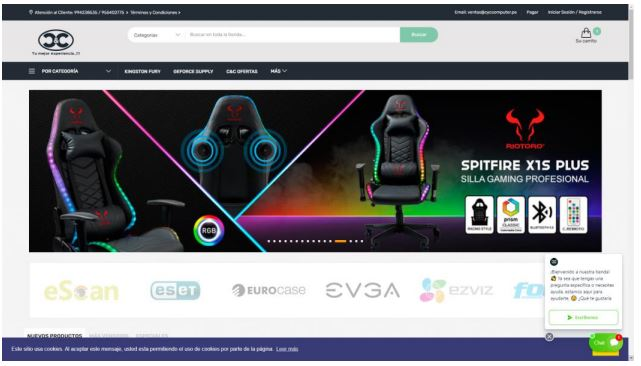
\includegraphics[width=5cm, height=3cm]{figuras/3.JPG}
      \caption{Página principal de la web e-commerce de la empresa C\&C Computer.}
      \label{f3} 
      \end{center}
\end{figure}
\end{enumerate} 
%---------------------------------------------------------------------------
\subsection{\underline{\textbf{Gestión de datos e información}}}
De acuerdo a \citep{datos}, la gestión de datos es el proceso de ingestión, almacenamiento, organización y mantenimiento de los datos creados y recogidos por una organización. La administración eficaz de los datos es una parte vital para el despliegue de los sistemas informáticos que ejecutan las aplicaciones empresariales.

La gestión de datos e información posee los siguientes objetivos: 
\begin{itemize}
    \item Garantizar la integridad de los datos. Así como también, garantizar que sean accesibles al personal autorizado para analizarlos.
    \item Asegurar que dichos datos sean confiables, que estén completos y que aporten información útil.
    \item Disminuir riesgos de pérdidas de datos e información.
    \item Buscar el aumento de la eficiencia de los procesos empresariales. Esto como parte de la toma de decisiones basadas en información confiable.
\end{itemize}

A continuación, algunas investigaciones respecto al área de Gestión de datos e información:
\begin{enumerate}
\item En la Tesis \textit{“Diseño de una base de datos geográfica para el manejo de información de concesiones en una empresa minera peruana”} Ingeniería de Sistemas de Información y Gestión.  Universidad Científica del Sur. Lima-Perú; \citep{palomino} plantea el diseño de una base de datos geográfico para el manejo de la información asociada a las concesiones en una empresa minera, este tipo de base de datos permitirá integrar la información descriptiva y geográfica en un único modelo de datos.  Al finalizar el diseño de la base de datos se obtuvo una estructura de datos que soporta el manejo de información descriptiva y geográfica que puede ser utilizado por diferentes aplicaciones y usuarios que requieran explotar la información de las concesiones mineras, además que el acceso y la gestión de la información es más eficiente.
\item En la investigación \textit{“Recolección de energía usando una Rectenna de bajo costo para aplicaciones de Internet de las cosas (IoT)”} Ingeniería de Sistemas. Universidad Nacional del Altiplano. Puno-Perú; \citep{condori} tuvo como objetivo general determinar si el Sistema de Información ayuda a la gestión del seguimiento de egresados. Para el desarrollo del sistema se utilizó la metodología Extreme Programming que es la metodología más destacada de los procesos ágiles de desarrollo de software.El sistema de Información contiene datos sobre experiencia laboral, estudios realizados, por lo que se verifico que el sistema si ayuda a la Gestión del Seguimiento de Egresados.
\begin{figure}[H]
 \begin{center}
       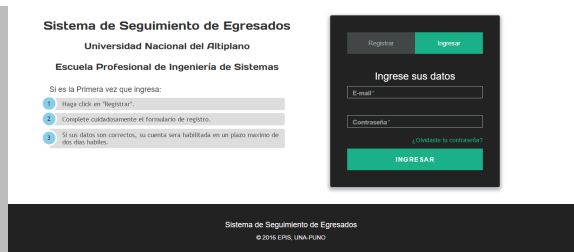
\includegraphics[width=5cm, height=3cm]{figuras/4.JPG}
      \caption{Pantalla de Inicio de Sistema de Seguimiento de Egresados.}
      \label{f4} 
      \end{center}
\end{figure}
\item En la investigación titulada \textit{“Diseño de un modelo de sistema integrado de infraestructura de red de datos para mejorar la gestión de la información en la Municipalidad Distrital de Mariscal Cáceres”} Maestría en Ingeniería de sistemas. Universidad Nacional del Centro del Perú. Huancayo-Perú; \citep{pacheco} se diseño un modelo de un Sistema Integrado de Infraestructura de Red de Datos, que integro la infraestructura de red de voz y la infraestructura de red de datos que actualmente son completamente independientes, y brindo seguridad a los datos y mejoro la gestión de la información en el Municipio.  La investigación se realizó en base a la metodología Top-Down de Cisco, identificando y analizando la situación de la infraestructura actual, llegándose a identificar las necesidades y dificultades en la administración de la red de datos, falta de seguridad y riesgos a los que está expuesto la red. 
\end{enumerate}
%---------------------------------------------------------------------------
\subsection{\underline{\textbf{Sistemas Inteligentes (IA)}}}
Los sistemas inteligentes son máquinas tecnológicamente avanzadas que perciben y responden al mundo que les rodea. Los sistemas inteligentes pueden tomar muchas formas, desde aspiradoras automáticas como Roomba hasta programas de reconocimiento facial y sugerencias de compras personalizadas de Amazon.\citep{systems}
\par El campo de los sistemas inteligentes también se enfoca en cómo estos sistemas interactúan con los usuarios humanos en entornos físicos y sociales cambiantes y dinámicos. Los primeros robots poseían poca autonomía para tomar decisiones: asumían un mundo predecible y perfumaban las mismas acciones repetidamente en las mismas condiciones. Hoy en día, se considera que un robot es un sistema autónomo que puede sentir el entorno y puede actuar en un mundo físico para lograr algunos objetivos.
\par A continuación, algunas investigaciones respecto a esta área de Sistemas Inteligentes:
\begin{enumerate}
\item En la tesis \textit{“Sistema inteligente conversacional para la orientación de internas con problemas familiares, en el Hogar Virgen de F\'atima de la Ciudad de Puno – 2013”} Ingeniería de Sistemas. Universidad Nacional del Altiplano. Puno-Perú; \citep{godoy} desarrollo el Sistema Inteligente Conversacional en la institución Hogar Virgen de F\'atima, para lo cual se necesitaba un agente inteligente (Figura ~\ref{f5}) que pueda conversar con las internas. Luego se diseñó las formas de interacción de las internas con el agente inteligente conversacional y las formas de aprendizaje que va a utilizar. Posteriormente, se implementó el sistema inteligente conversacional basada en el lenguaje de programación Java, logrando conversar con las internas dando buenos consejos para su posterior desarrollo en su vida y además identificando el tipo de problema familiar que poseen.
\begin{figure}[H]
 \begin{center}
       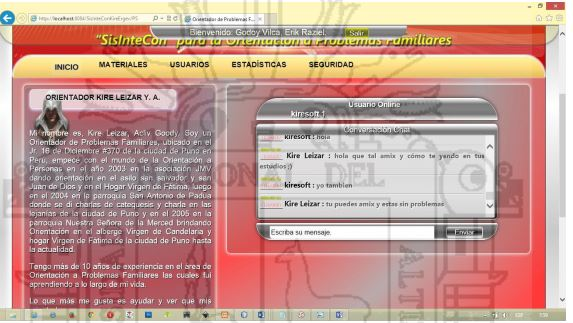
\includegraphics[width=7cm, height=4cm]{figuras/5.JPG}
      \caption{ Diseño de interfaz de Conversación con el agente Inteligente}
      \label{f5} 
      \end{center}
\end{figure}
\item En la tesis \textit{“Sistema inteligente para rotación de personal basado en algoritmos genéticos en la empresa Soluciones TEC Perú”} Ingeniería de Sistemas. Universidad César Vallejo. Lima-Perú; \citep{rivera} para el desarrollo del sistema inteligente, se empleó la metodología COMMONKADS, por ser la que más se acomodaba a las necesidades y etapas del proyecto, además por ser rápida en tiempos de entrega, de esta manera no se generó resistencia al cambio en los usuarios. La implementación del Sistema inteligente permitió aumentar la eficacia del 40,78\% a 74,02\%, del mismo modo, se aumentó la eficiencia del 32,25\% al 90,31 \%. Los resultados mencionados anteriormente, permitieron llegar a la conclusión que el sistema inteligente mejora la rotación de personal basado en algoritmos genéticos en la empresa Soluciones TEC Perú.
\begin{figure}[H]
 \begin{center}
       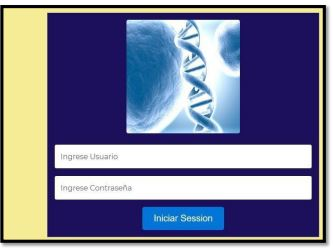
\includegraphics[width=7cm, height=4cm]{figuras/6.JPG}
      \caption{ Pantalla de inicio del Sistema Inteligente}
      \label{f6} 
      \end{center}
\end{figure}
\item En la tesis \textit{“Análisis y diseño de un Sistema de Control de Trafico Vehicular Utilizando Semáforos Inteligentes con Tecnología Arduino”} Ingeniería Electrónica. Universidad Nacional del Altiplano. Puno-Perú; \citep{machaca} basa la metodología para el desarrollo del sistema en el Microcontrolador Arduino por medio de procesamiento digital de imágenes programado en Matlab de manera inteligente con algoritmos para la toma de decisiones en el área del control de tráfico vehicular. El desarrollo del sistema está constituido por cámaras que adquieren imágenes y envía las imágenes para el procesamiento digital de imágenes usando un software llamado Matlab, la densidad del tráfico vehicular se determina y el Microcontrolador cambia la duración de la luz verde dada para cada carretera según el número de vehículos existentes en la vía de tránsito.

\end{enumerate}








%---------------------------------------------------------------------------
\subsection{\underline{\textbf{Diseño de software}}}
La Universidad DeVry \citep{diseno} lo define como el \textbf{proceso que permite al usuario definir métodos y parámetros} de software. El diseño trabaja con funciones y la estructura general del código. Le permite preparar un plan para una aplicación de software mientras cumple con los requisitos funcionales y evita las limitaciones del programa.

Algunas de las habilidades que un diseñador de software utiliza en el trabajo pueden incluir:
\begin{itemize}
    \item Análisis de las necesidades de los usuarios.
    \item Evaluación de las necesidades/objetivos de la empresa
    \item Desarrollo del sistema de software dentro de los parámetros establecidos.
    \item Mantenimiento de sistemas de software para verificar la potencia continua
\end{itemize}

A continuación, algunas investigaciones respecto al área del diseño de software:

\begin{enumerate}
\item Los autores de \textit{"Diseño de software para control del proceso de cotizaciones en Pyme del cantón La Maná"} \citep{albarracin2022diseno}, en su investigación proponen introducir mejoras en el proceso de cotización en Pyme de venta de accesorios vehiculares del cantón La Maná, con la creación de un software para esta finalidad, obsérvese Figura ~\ref{fmana}. Se utilizaron métodos como el analítico-sintético, inductivo-deductivo y sistemático. Se aplicó una encuesta, a una muestra de 172 directivos, empleados y clientes, obteniéndose como resultado que la utilización de un software beneficia el proceso de cotización y que la aplicación de las nuevas tecnologías influye de manera positiva en la gestión de las Pyme.

\begin{figure}[H]
 \begin{center}
       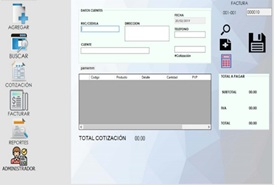
\includegraphics[width=7cm, height=4cm]{figuras/mana.JPG}
      \caption{Interfaz del Menú Programa Visual Studio 2015.}
      \label{fmana} 
      \end{center}
\end{figure}

\item La investigación \textit{"Propuesta de diseño de software con código QR para la gestión del inventario de la empresa 'Vamos Supermercado' S.R.L."} \citep{albarracin2022diseno}, obtuvo como resultado una gestión de inventario con código QR (ver Figura ~\ref{fqr}), herramientas afines para el análisis de mercado de la empresa, modelado del negocio, diseño de la marca y nombre, así como su análisis económico financiero. Inicialmente la empresa brindó información para que se conozca el alto índice de manualidad en el proceso de gestión de inventarios. Por lo que se digitalizó y sistematizó y el diseño del sistema fue desarrollado por MySQL Workbench para el modelado relacional de la base de datos, Justinmind para el diseño de las interfaces gráficas y el aplicativo web Lucidchart para la generación de los diagramas para el análisis. 

\begin{figure}[H]
 \begin{center}
       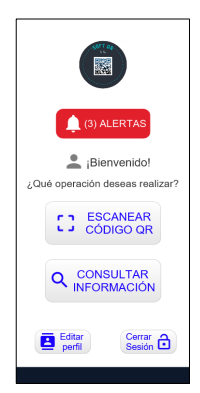
\includegraphics[width=4cm, height=5cm]{figuras/qr.PNG}
      \caption{Pantalla principal en aplicativo móvil del software con código QR.}
      \label{fqr} 
      \end{center}
\end{figure}

\item Otra investigación es \textit{“El diseño de software de Gridap: un paquete de elementos finitos basado en el compilador Julia JIT”} \citep{VERDUGO2022108341}, donde se expone el diseño de software de Gridap, una novedosa biblioteca, que simula fenómenos físicos complejos como magnetohidrodinámica, fotónica, modelado meteorológico, sólidos no lineales, mecánica y problemas de interacción fluido-estructura. La principal contribución de este artículo es el detalle de las abstracciones de software detrás del diseño de Gridap que aprovecha las posibilidades de software proporcionadas por el lenguaje Julia. La segunda contribución principal es una comparación de rendimiento frente a FEniCS, lo que demuestra que el nuevo diseño de software no compromete el rendimiento.
\end{enumerate}
%---------------------------------------------------------------------------
\subsection{\underline{\textbf{Gráficos y Visualización}}}
Según la Universidad de Oregon \citep{gradef}, los gráficos y visualización por computadora están formados por el procesamiento de imágenes, análisis visual, programación de GPU, simulación y procesamiento de geometría. Los objetivos principales son:
\begin{itemize}
    \item El análisis, la síntesis, la comprensión y la manipulación de datos visuales como imágenes, secuencias de video y contenido geométrico en 3D.
\end{itemize}
Las áreas de aplicación abarcan una amplia gama, desde entretenimiento artístico hasta ciencia e ingeniería, biología y medicina.

Algunas investigaciones respecto al área de Gráficos y Visualización por computadora:

\begin{enumerate}
\item El estudio \textit{“Análisis bibliométrico de visualizaciones en gráficos por computadora: un estudio"} \citep{bio}, examinó el campo de las visualizaciones en gráficos por computadora (VCG) utilizando métodos bibliométricos, incluido el análisis de mapeo científico, ver Figura ~\ref{fbio} y de rendimiento. Se analizó y visualizó un conjunto de datos de documentos de SCOPUS, de 1986 a 2019, utilizando VOSviewer. Los resultados mostraron una tendencia creciente de nuevos documentos en VCG. Las cinco publicaciones más citadas estaban todas relacionadas con el software de visualización de datos, contribuyendo en la investigación en gráficos por computadora, visualización de información, análisis de datos interactivos, interfaces hombre-computadora y desarrollo de software de visualización.

\begin{figure}[H]
 \begin{center}
       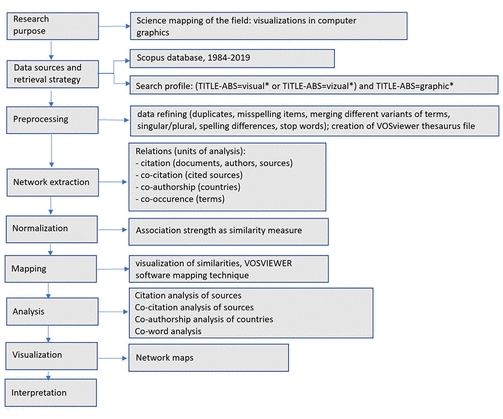
\includegraphics[width=7cm, height=5cm]{figuras/bio.PNG}
      \caption{Flujo de trabajo del mapeo científico aplicado en este estudio.}
      \label{fbio} 
      \end{center}
\end{figure}

\item El artículo titulado \textit{“Métodos de modelado de nubes atmosféricas en gráficos por computadora: una revisión, tendencias, taxonomía y direcciones futuras"} \citep{visu}, aborda que el modelado de nubes atmosféricas es uno de los elementos cruciales en el sistema de visualización de fenómenos naturales. Sin embargo, la falta de artículos de revisión sobre los métodos de modelado de nubes atmosféricas disponibles en gráficos por computadoras hace que sea difícil comprender y elegir las soluciones adecuadas. Por lo tanto, se llevo a cabo una revisión integral para identificar, analizar, clasificar y resumir las soluciones de modelado de nubes atmosféricas existentes. Finalmente, se seleccionó 113 estudios de investigación de fuentes de datos reconocibles y se analizó las tendencias de investigación sobre este tema. 

\item La tesis titulada \textit{“Generación automática de casos de prueba para test de una GUI, usando colonia de hormigas y metaheurística golosa“}, presenta una propuesta del uso de dos metaheurísticas, las que permitirán la generación automática de casos de prueba para test sobre una GUI (Graphical User Interface), Interfaz gráfica del usuario, usando un conjunto de imágenes y objetos gráficos para representar la información y acciones disponibles en la interfaz, con el objetivo de que sean aplicados al producto final (pruebas funcionales) y detecten en qué puntos el producto no cumple sus especificaciones. Esto facilitará a las empresas de software la modificación de algún artefacto o componente del sistema por cambios en el negocio.

\end{enumerate}

%---------------------------------------------------------------------------
\subsection{\underline{\textbf{Arquitectura y Organización}}}
Como lo manifiestan \citep{bookar} una arquitectura es un modelo de sistema dentro de un contexto específico, que representa los componentes necesarios para desarrollar el sistema desde una perspectiva o punto de vista particular. Mientras que la organización básica de una computadora consiste en la unidad de entrada, por medio de la cual se introducen datos e instrucciones; la unidad central de procesamiento, donde se procesan los datos de acuerdo con las instrucciones dadas, y la unidad de salida, por medio de la cual se presenta la información resultante al usuario.

A continuación, algunas investigaciones respecto al área de arquitectura y organización de computadores:

\begin {enumerate}
\item La tesis de la Universidad Científica del Sur con el título\textit{"Diseño de una arquitectura de seguridad informática para incrementar la seguridad de información en la empresa Bafing S.A.C. en 2021"} \citep{asurza2022diseno}, tiene carácter experimental, donde para llevar a cabo dicho propósito se evaluaron propuestas de software de seguridad, ver Figura ~\ref{farq}, objetivo seleccionado bajo un perfil y se juzgó cada uno de ellos confrontando sus resultados en función al cumplimiento de la integridad, confidencialidad y disponibilidad. Las herramientas de evaluación usadas en el proyecto fueron colectadas a partir de la información de entrevistas con especialistas en el rubro de protección de información y activos informáticos. Los resultados obtenidos mostraron mejoras en las dimensiones de seguridad de información analizadas respecto a la situación actual de la empresa auditada BAFING S.A.C.

\begin{figure}[H]
 \begin{center}
       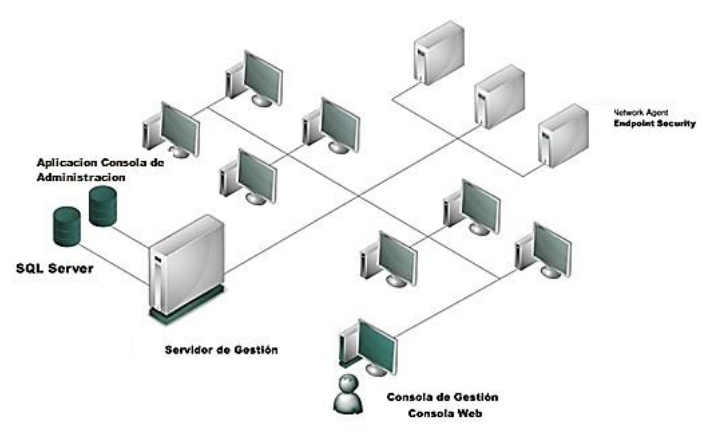
\includegraphics[width=7.5cm, height=5cm]{figuras/arq.PNG}
      \caption{Propuesta de Solución: Modelo de Arquitectura de Seguridad informática Empresa BAFING S.A.C.}
      \label{farq} 
      \end{center}
\end{figure}

\item La investigación \textit{"Diseño de una arquitectura de computadoras de propósito didáctico"} \citep{upm69893}, se llevo a cabo como una extensión de las asignaturas de fundamentos, estructura, y arquitectura de computadores. Además, se diseño una arquitectura de computador reducida. Esto se realiza a nivel conceptual mediante el diseño de los componentes como una caja negra con entradas y salidas, a nivel estructural viendo el interior de cada componente formado por puertas lógicas, y a nivel de implementación modelándolos en VHDL, un lenguaje de descripción hardware. Como resultado se menciona que a diferencia de estudiar una arquitectura ya creada, observar su desarrollo o desarrollar una desde cero aporta la visibilidad necesaria para captar la complejidad y detalle de todas sus partes, ofreciendo al estudiante una perspectiva global muy útil.

\item La tesis de titulación \textit{"Implementación de una arquitectura de red, como aporte a la gestión de seguridad informática del Hotel San Pablo de la provincia de Santa Elena, Ecuador."} \citep{alvarez2022implementacion}, su propósito es ofrecer a los usuarios una óptima y eficiente conectividad al servicio de internet. Siendo de enfoque cualitativo, la implementación de la arquitectura de red utilizó la metodología PPDDIO, obsérvese Figura ~\ref{fhot}, cuyo objetivo es optimizar el desempeño a través del ciclo de vida de la red. Se empleó la topología de red en estrella, estableciendo así el dispositivo principal de gestión red, Routerboard. Permitiendo gestionar y administrar la red informática implementada con la herramienta de interfaz gráfica que ofrece la aplicación Winbox del equipo mikrotik. Las pruebas realizadas demuestran que el proyecto es factible y viable para implementaciones de redes privadas virtuales.

\begin{figure}[H]
 \begin{center}
       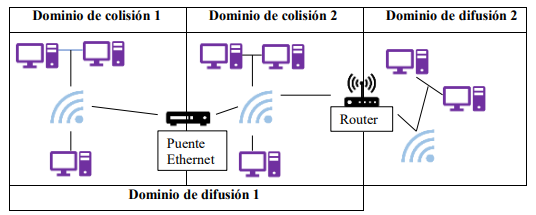
\includegraphics[width=8cm, height=5cm]{figuras/hotel.PNG}
      \caption{Arquitectura de Ethernet. Metodología PPDDIO}
      \label{fhot} 
      \end{center}
\end{figure}


\end{enumerate}
%---------------------------------------------------------------------------
\section{\textbf{Conclusión}}
Este informe presentó información relevante acerca de seis áreas de ciencias de la computación basado en la Computing Curricula 2020, se ha explicado los conceptos teóricos relacionados con ellas. Además de permitir conocer sobre algunas investigaciones que se vienen realizando año a año, entendiendo las diversas aplicaciones de las ciencias de la computación en la vida diaria. Concluimos respecto a ello que la mayoría analiza el proceso y propone resolver problemas utilizando soluciones técnicas, por la que este es un campo tan importante donde se evidencia que las computadoras y la tecnología se han integrado en prácticamente todos los sectores educación, económicos, industrias e incluso organizaciones que operan en la economía moderna.
%-------------------------------------------------------
\medskip
\bibliography{refer}
\end{document}